\documentclass[10pt,utf8]{beamer}

\mode<presentation> {
  \usetheme{Madrid}
  \setbeamercovered{transparent}
}

\usepackage{palatino}
\usepackage{graphicx}
\usepackage{array}
\usepackage{color}
\usepackage{subfigure}
\usepackage{colortbl}
\usepackage{amsmath}
\usepackage{hyperref}
\usepackage{listings}
\usepackage{fancyvrb}

\setbeamertemplate{caption}{\raggedright\insertcaption\par} %turn off caption prefix ("Figure")

\definecolor{delim}{RGB}{20,105,176}
\definecolor{numb}{RGB}{106, 109, 32}
\definecolor{string}{rgb}{0.64,0.08,0.08}

\title{Vector databases}
\author{Vojtěch Juránek}
\institute[IBM]{IBM}
\date{September 22nd 2025, RH CZ AI Buddy, Brno}

\newenvironment{mylisting}
{\begin{list}{}{\setlength{\leftmargin}{1em}}\item\scriptsize\bfseries}
{\end{list}}

\newenvironment{mytinylisting}
{\begin{list}{}{\setlength{\leftmargin}{1em}}\item\tiny\bfseries}
{\end{list}}


\begin{document}

\begin{frame}
    \titlepage
\end{frame}

\begin{frame}
    \frametitle{Vector database}
    \begin{itemize}
        \item Designed to store (high-dimensional) vectors.
        \item Effective search capabilities for similar vectors.
        \item Allow to store also vector metadata and/or original object from which the vector was derived.
    \end{itemize}
\end{frame}

\begin{frame}
    \frametitle{Vector embedding}
    \begin{itemize}
        \item Input data (text, audio, video) is transformed to high-dimensional vector by embedding model/transformer.
        \item Embedding captures some properties (usually semantics meaning) of the input data.
        \item Allows to do a similarity search across set of the vectors.
    \end{itemize}
    
    \vspace{0.1cm}
    
    \begin{figure}
        \centering
        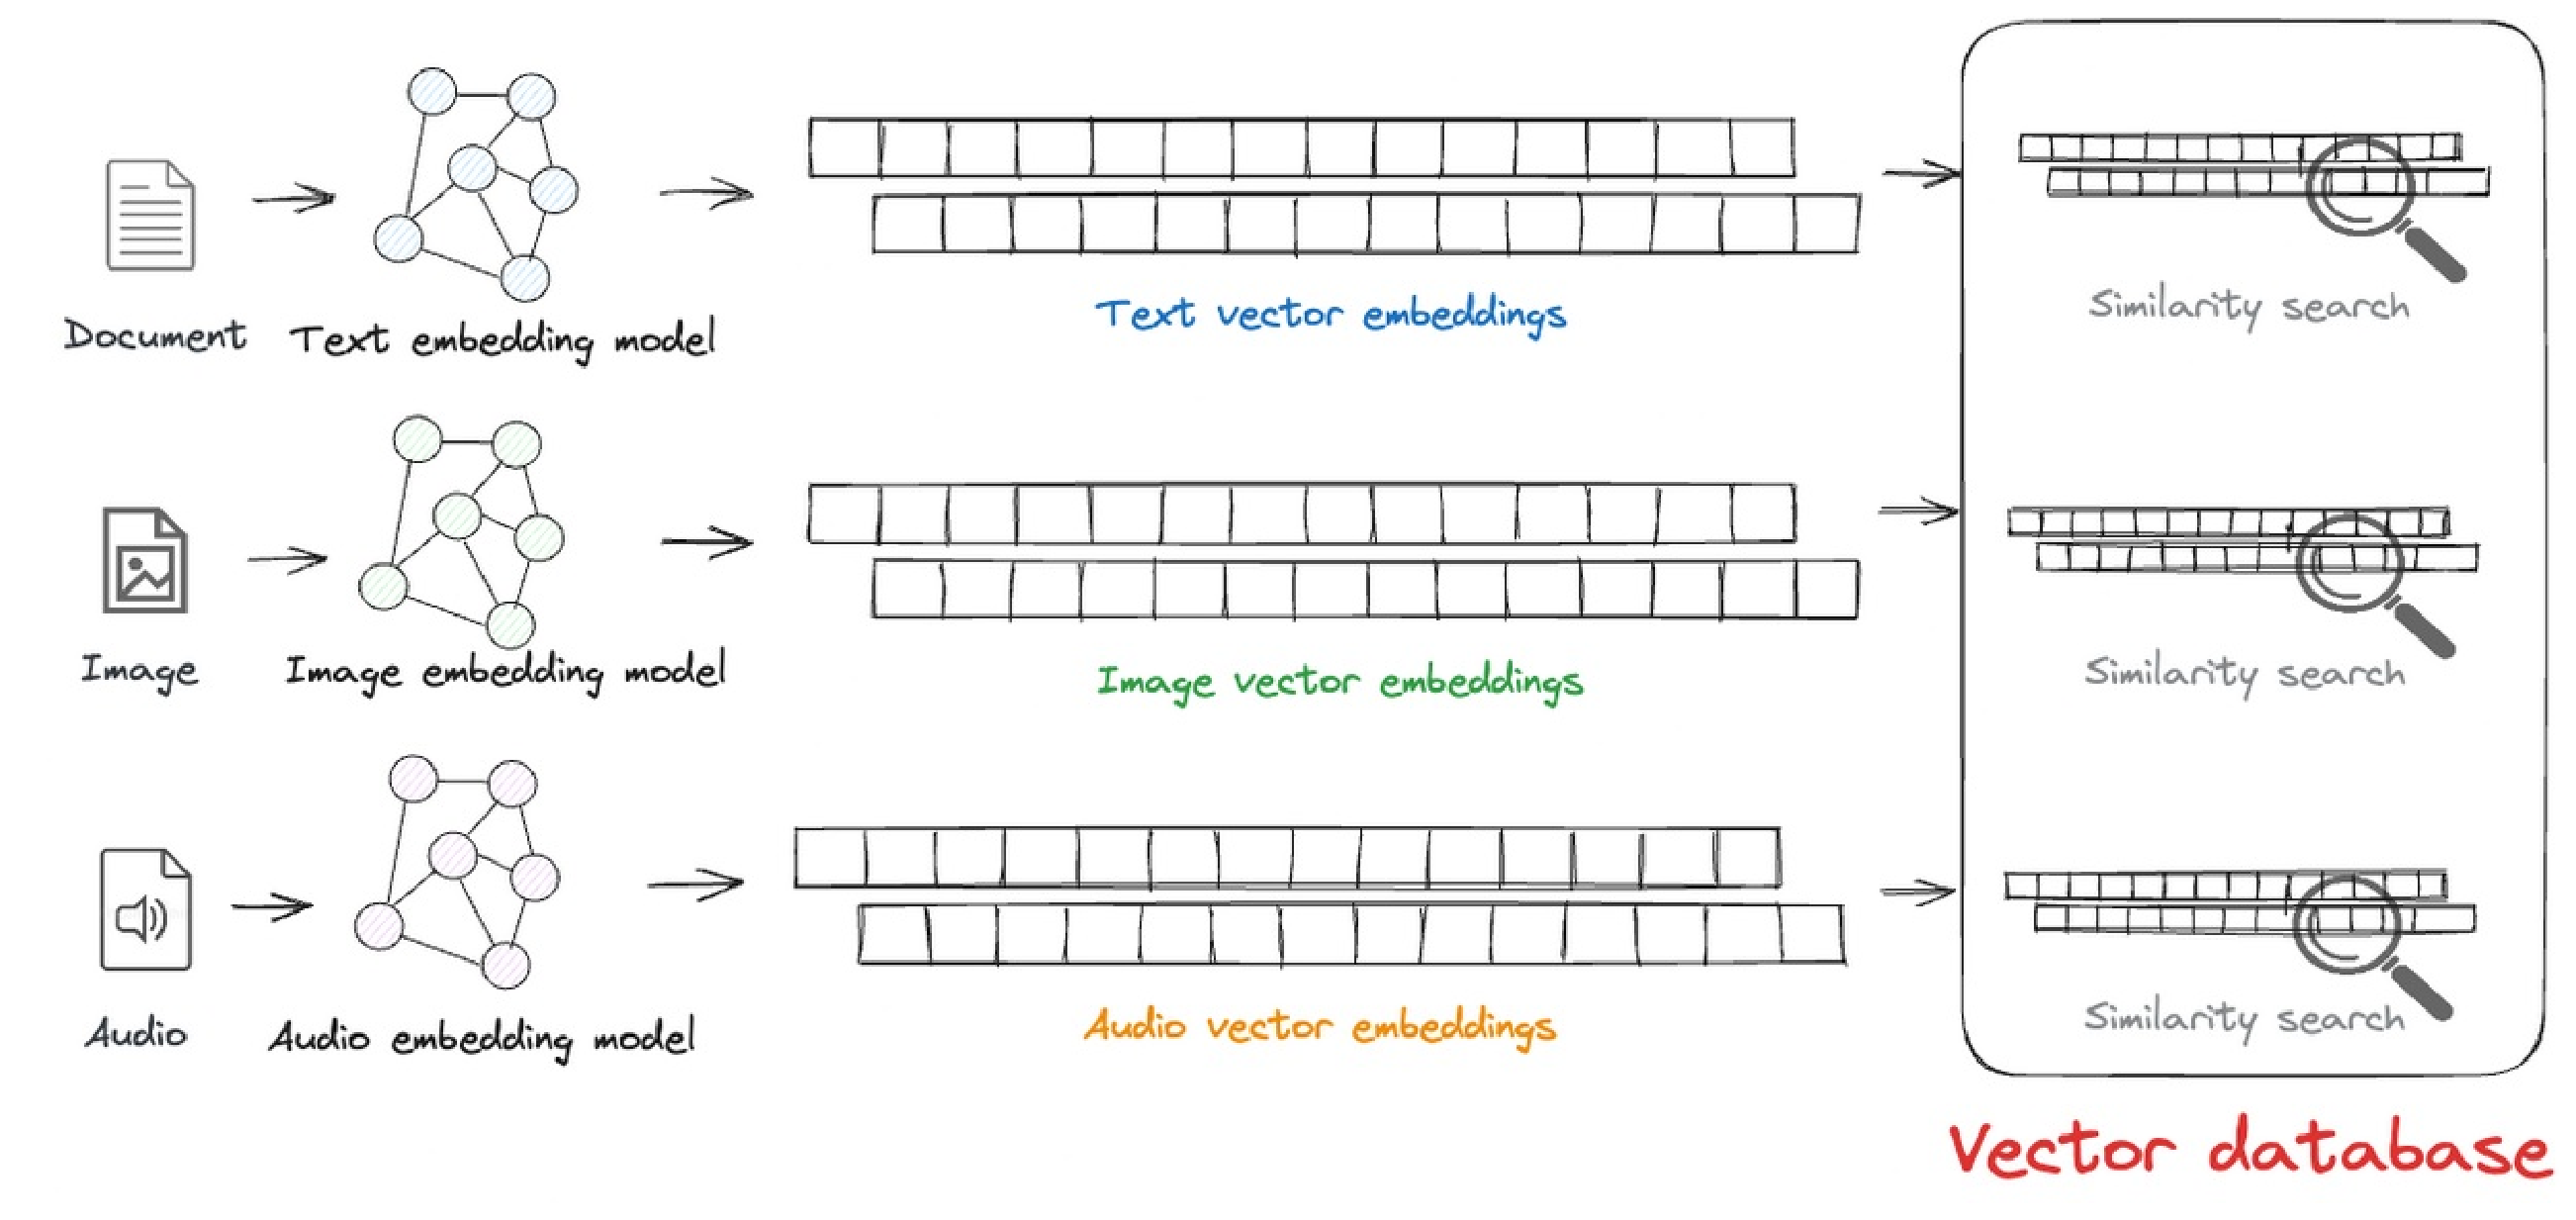
\includegraphics[height=5cm]{./img/media_to_db.eps}
        \caption{\tiny{Source: \url{https://thedataquarry.com/blog/vector-db-2/}}}
    \end{figure}
\end{frame}

\begin{frame}
    \frametitle{Vector embedding}
    \begin{itemize}
        \item Similar embeddings correspond to objects which are also \textbf{semantically} similar.
        \item Vector embeddings have other interesting properties, e.g. well know 
        \begin{equation}
            % \boxed{king - man + woman \approx queen}
            king - man + woman \approx queen
        \end{equation}
    \end{itemize}
\end{frame}

\begin{frame}
    \frametitle{Metric types}
    To be able to do similarity search, we have to define how to measure similarity - we have to define metric on given vector space.
    
    \vspace{0.1cm}
    
    \begin{itemize}
        \item Metric measure the distance of two vectors.
        \item It express similarity among the vectors.
        \item Usually smaller distance means bigger similarity, but there are also metrics where bigger number means bigger similarity.
    \end{itemize}
\end{frame}

\begin{frame}
    \frametitle{Metric examples}
    \begin{itemize}
        \item L2 (Euclidian) $$d(x,y) = \sqrt{\sum_{i=1}^{n} (x_i - y_i)^2}$$
        \item L1 (Manhattan) $$d(x,y) = \sum_{i=1}^{n} |x_i - y_i|$$
        \item scalar/inner product (vector need to be normalized) $$x \cdot y = \sum_{i=1}^{n} x_i \cdot y_i$$
        \item cosine similarity $$\cos{\Theta} = \frac{x \cdot y}{|x||y|}$$
        \item Jaccard index (similarity of two sample sets) $$J(A, B) = \frac{|A \cap B|}{|A| + |B| - |A \cap B|}$$
    \end{itemize}
\end{frame}

\begin{frame}
    \frametitle{Vector index}
    \begin{itemize}
        \item Enabled effective \textbf{similarity} search in high-dimensional vector space.
        \item As in relational DB, updating index adds overhead during data insertion.
        \item Some index types sacrifice precision for speed.
    \end{itemize}
\end{frame}

\begin{frame}
    \frametitle{Vector indexes examples}
    \begin{itemize}
        \item Inverted file (IVF)
            \begin{itemize}
                \item Splits data into several clusters using e.g. K-means clustering.
                \item Query identifies the most similar cluster and search only this cluster.
                \item Has many variants like IVFFlat, IVFPQ (IVF product quantization), \dots
            \end{itemize}
            \vspace{0.2cm}
        \item Locality-sensitive hashing (LSH)
            \begin{itemize}
                \item Hash-based algorithm,  vectors are clustered based on the fuzzy hashing function.
            \end{itemize}
            \vspace{0.2cm}
        \item Hierarchical Navigable Small World (HNSW)
            \begin{itemize}
                \item Graph-based algorithm, nearest neighbours are connected.
                \item Index organized in several layers, higher level are more sparse.
            \end{itemize}
    \end{itemize}
\end{frame}

\begin{frame}
    \frametitle{HSNW search}
    \vspace{-0.5cm}
    \begin{figure}
        \centering
        
\includegraphics[height=7cm]{./img/hnsw_search.eps}
        \caption{\tiny{Source: \url{https://docs.weaviate.io/weaviate/concepts/vector-index}}}
    \end{figure}
\end{frame}

\begin{frame}
    \frametitle{Popular vector database}
    \begin{itemize}
        \item All major relational databases now support vector data types and related functions.
        \item Major search engine supporting vectors
            \begin{figure}
                \centering
                
\includegraphics[height=1cm]{./img/search_engines.eps}
            \end{figure}
        \item Specialized vector database
            \begin{figure}
                \centering
                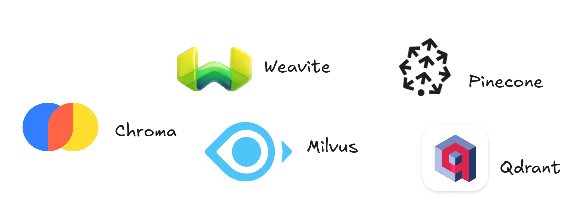
\includegraphics[height=3cm]{./img/vector_databases.eps}
            \end{figure}
        \item And many more \dots
    \end{itemize}
\end{frame}

\begin{frame}[fragile]
    \frametitle{Vector Database Demo - pgvector}
    \begin{mylisting}
        \begin{lstlisting}
docker run --rm --name postgres -e POSTGRES\_PASSWORD=postgres -d -it -p 5432:5432 quay.io/debezium/postgres:17 \\
PGPASSWORD=postgres psql -h localhost -U postgres postgres
        \end{lstlisting}
    \end{mylisting}

    \vspace{0.5cm}
    
    \begin{mylisting}
        \begin{lstlisting}
CREATE EXTENSION IF NOT EXISTS vector;
CREATE TABLE vect_test (id serial PRIMARY KEY, embedding vector(3));
INSERT INTO vect_test(embedding) VALUES ('[1,1,1]'), ('[2,2,2]'), 
('[3,3,3]'), ('[4,4,4]'), ('[5,5,5]'), ('[5,5,6]'), ('[5,6,5]');
SELECT * FROM vect_test ORDER BY embedding <-> '[5,5,5]' limit 3;
SELECT * FROM vect_test WHERE embedding <->  '[5,5,5]' < 2
SELECT * FROM vect_test WHERE embedding <+>  '[5,5,5]' < 2;
SELECT * FROM vect_test WHERE embedding <=>  '[5,5,5]' = 0;
        \end{lstlisting}
    \end{mylisting}
\end{frame}

\begin{frame}
    \frametitle{Retrieval Augmented Generation (RAG)}
    \begin{itemize}
        \item Provides LLM accurate and relevant information for generating the response.
        \item Leverages external data source.
        \item Complementary strategy to LLM fine tuning how to improve relevance of the LLM's answers.
    \end{itemize}
    \begin{figure}
        \centering
        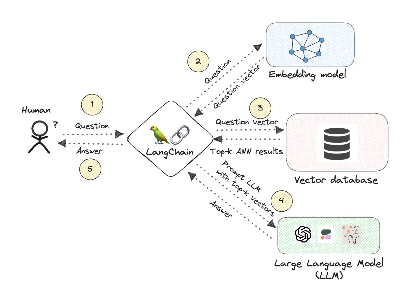
\includegraphics[height=5cm]{./img/rag.eps}
        \caption{\tiny{Source: \url{https://thedataquarry.com/blog/vector-db-2/}}}
    \end{figure}
\end{frame}

\begin{frame}
    \begin{figure}
        \centering
        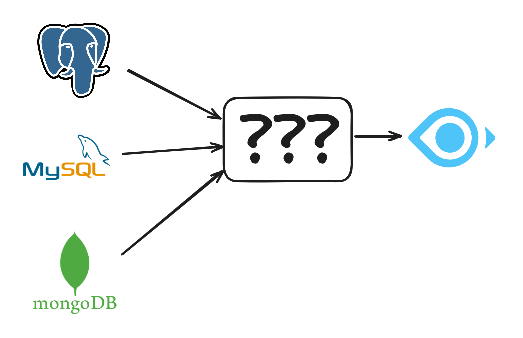
\includegraphics[height=7cm]{./img/db_to_milvus.eps}
    \end{figure}
\end{frame}

\begin{frame}
    \begin{figure}
        \centering
        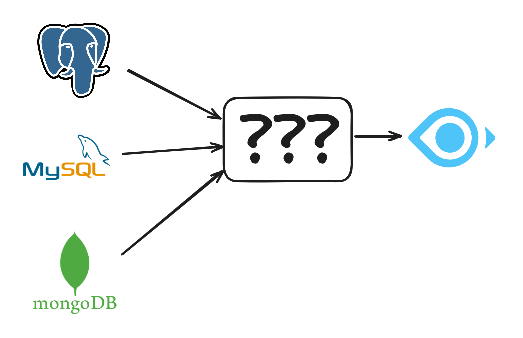
\includegraphics[height=4cm]{./img/db_to_milvus.eps}
    \end{figure}
    \begin{itemize}
      \item Consistent data, no data losses, no dual writes.
      \item Get all the changes without any delay in the real-time.
      \item Not overload the DB with the queries.
    \end{itemize}
\end{frame}

\begin{frame}
    \begin{figure}
        \centering
        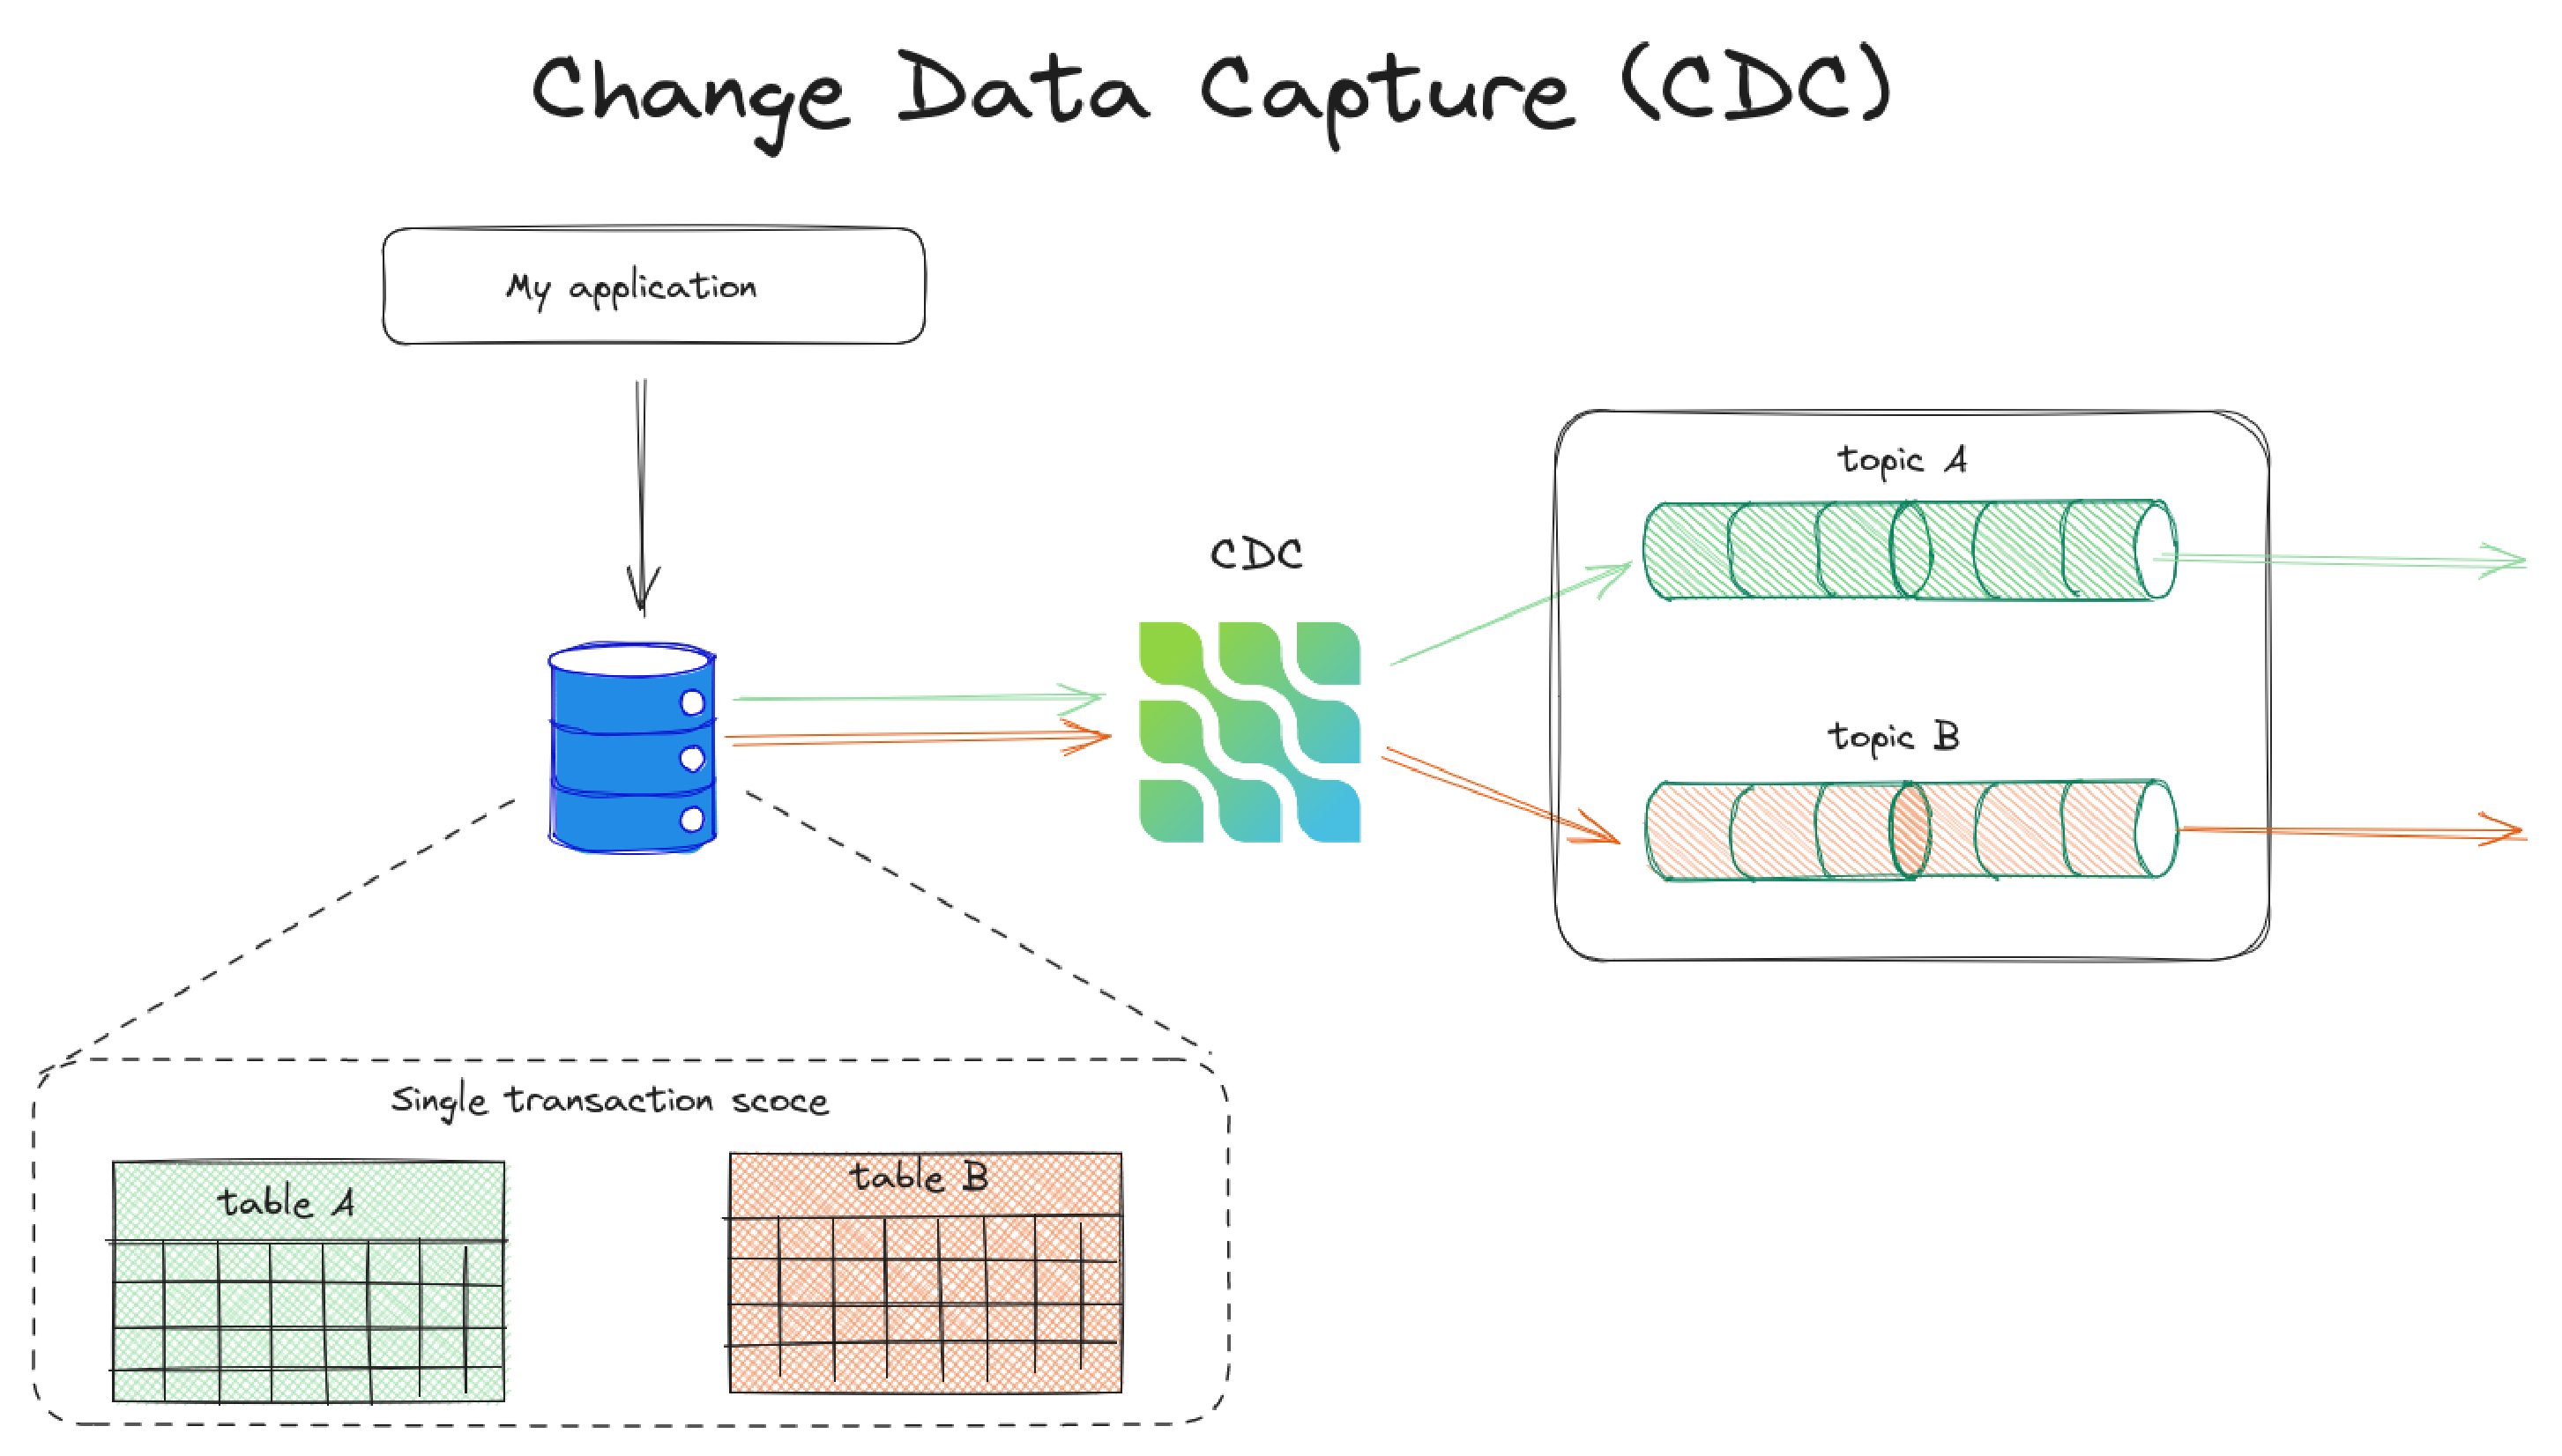
\includegraphics[height=7cm]{./img/cdc.eps}
    \end{figure}
\end{frame}

\begin{frame}
   \frametitle{Debezium}
   \begin{figure}
        \centering
        
\includegraphics[height=1.5cm]{./img/debezium.eps}
    \end{figure}
    
    \vspace{0.5cm}
    
   \begin{itemize}
     \item Leading CDC framework, de-facto industry standard.
     \item Fully open source: \textcolor{blue}{\url{https://github.com/debezium/}}
     \item Supports all major databases, including non-relational databases.
     \item Integrations with many 3rd-party tools and frameworks.
     \item Large and active user community.
     \item Used by many companies in production (see \textcolor{blue}{\href{https://debezium.io/community/users/}{Debezium public references}}).
   \end{itemize}
\end{frame}

\begin{frame}
    Debezium can be deployed as
    \begin{itemize}
        \item Kafka source connector
        \item standalone server
        \item library which can be embedded into Java application
    \end{itemize}
    
    \begin{figure}
        \centering
        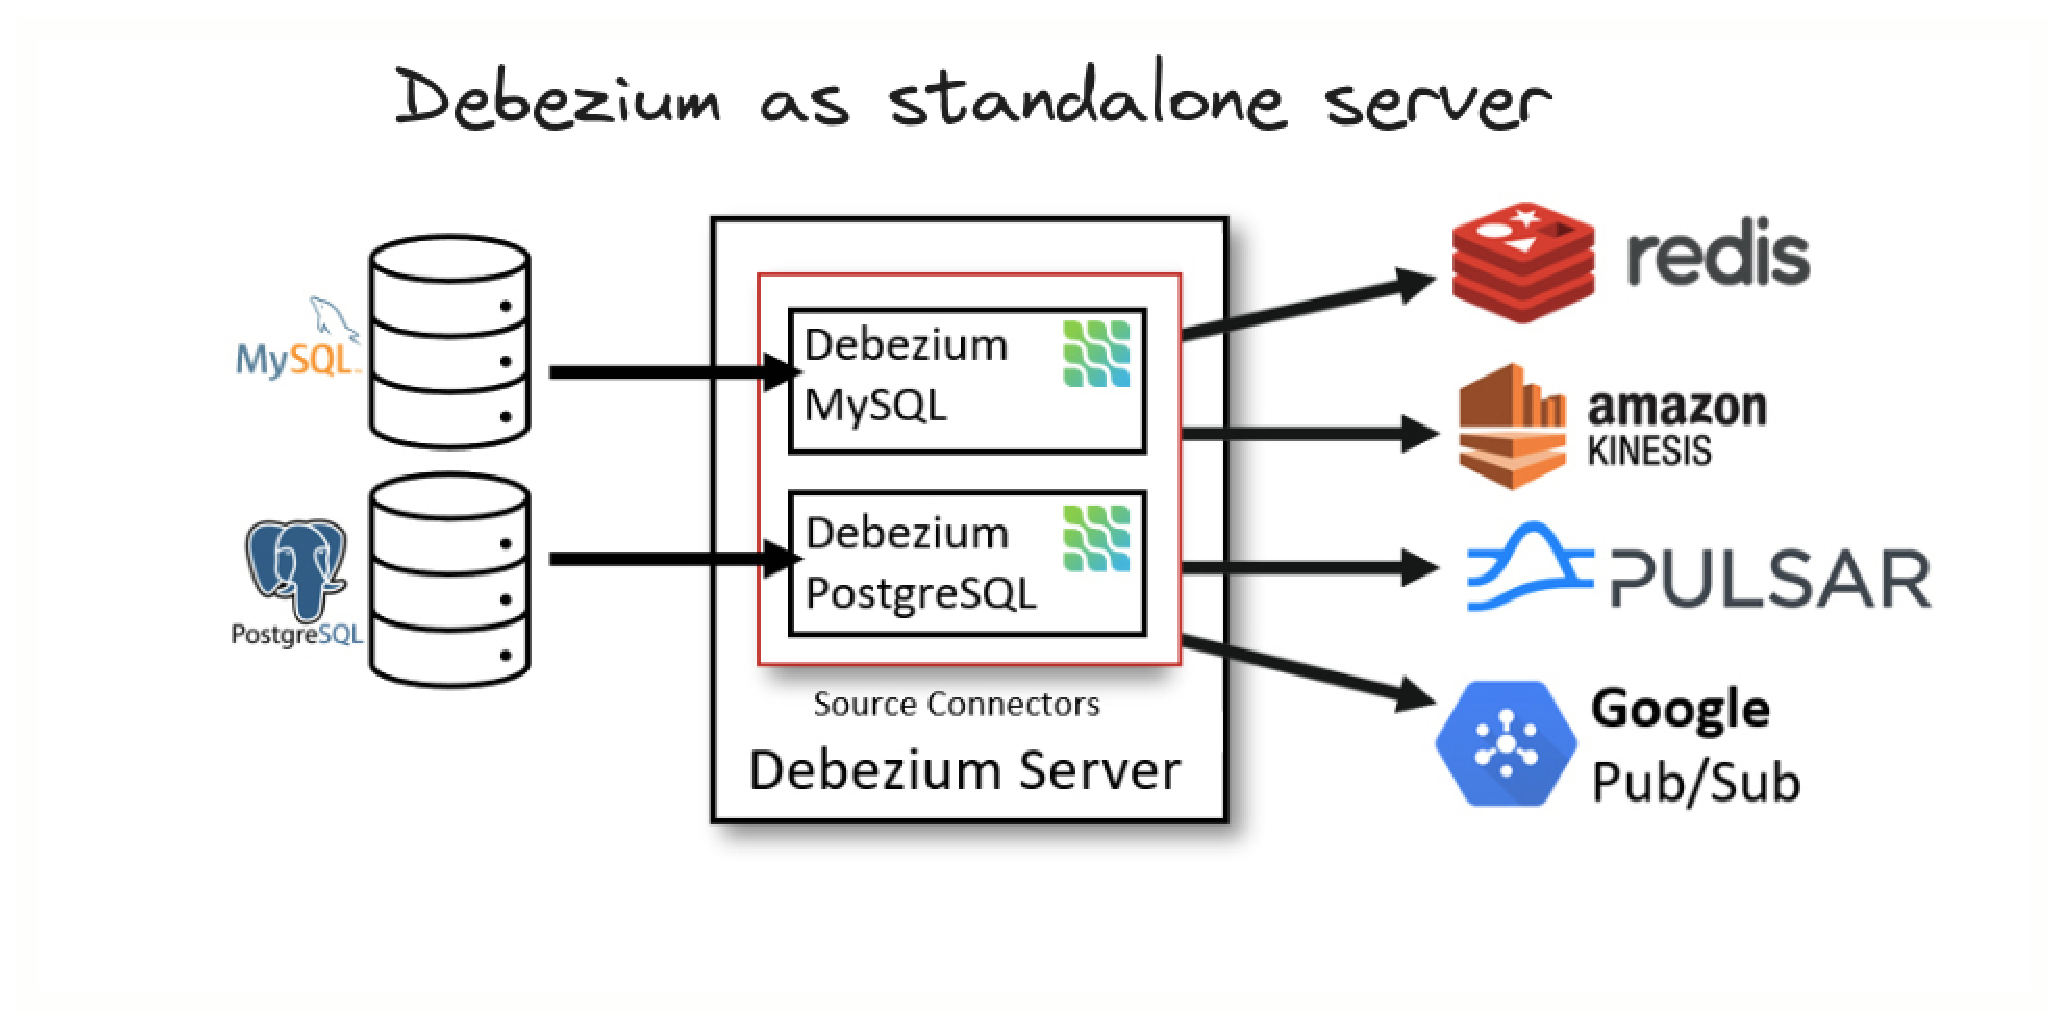
\includegraphics[height=6cm]{./img/debezium_server.eps}
    \end{figure}
\end{frame}

\begin{frame}
     \frametitle{RAG with Debezium}
     \begin{itemize}
        \item Debezium provides AI module which allows to create embeddings as a single message transform (SMT).
        \item Integrated with major LLM provides.
        \item Currently Debezium server provides direct integration with Milvus, Qdrant and InstructLab.
        \item For Kafka Connect we provide JDBC sink connector, also dedicated Kafka Connect sink connectors for Milvus and others exists.
        \item No need to do any changes to the legacy applications or adjusting data flows.
        \item Modernization of the app stack can happen in parallel to existing applications without any distraction.
     \end{itemize}
\end{frame}

\begin{frame}
    \frametitle{RAG Demo: PostgreSQL, Debezium, Milvus}
    See
    \begin{itemize}
        \color{blue} \footnotesize
        \item \url{https://github.com/debezium/debezium-examples/tree/main/ai-rag}
        \item \url{https://debezium.io/blog/2025/05/19/debezium-as-part-of-your-ai-solution/}
        \color{black}
    \end{itemize}
    \begin{figure}
        \centering
        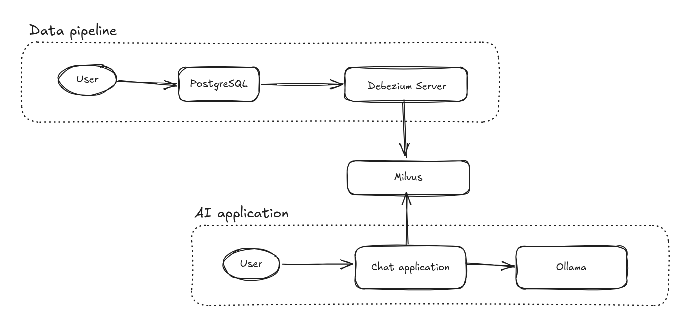
\includegraphics[height=5cm]{./img/dbz_milvus_demo.eps}
        \caption{\tiny{Source: \url{https://debezium.io/blog/2025/05/19/debezium-as-part-of-your-ai-solution/}}}
    \end{figure}
\end{frame}

\begin{frame}
    \frametitle{Questions?}
    \centering
     \textbf{\Huge{Thank you!}}
    
    \vspace{1.5cm}
    
    \textbf{\Huge{Questions?}}
    
    \vspace{1cm}
\end{frame}

%%%%%%%%%%%%%%%%%%%%%%%%%%%%%%%%%%%%%%%%%%%%%%%%%%%%%%%%%%%%%%%%%%%%%%%%%%%%%%%%%%%%%%%%%%%%%%%%%
%%% BACKUP
%%%%%%%%%%%%%%%%%%%%%%%%%%%%%%%%%%%%%%%%%%%%%%%%%%%%%%%%%%%%%%%%%%%%%%%%%%%%%%%%%%%%%%%%%%%%%%%%%

\begin{frame}
    \centering
    \huge{\textbf{Backup slides}}
\end{frame}

\begin{frame}
    \frametitle{Product quantization}
    \begin{figure}
        \centering
        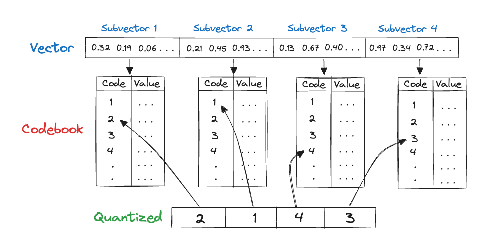
\includegraphics[height=5.5cm]{./img/product_quantization.eps}
        \caption{\tiny{Source: \url{https://lancedb.github.io/lancedb/concepts/index_ivfpq/}}}
    \end{figure}
\end{frame}

\end{document}
